The question explores whether the members should sign a capacity limitation contract with the DSO. To answer this, three different optimization models based on different contracts will be explored. In model $\mathcal{R}$, no contract is signed and each member schedules independently at the full tariffs. In model $\mathcal{I}$, each member signs its own contract with a share of the capacity limit. The trade-off is that members get lower tariffs for import and export but have to pay a penalty if they exceed the limit. In this model, each member still acts independently. The last model $\mathcal{C}$ is similar to model $\mathcal{I}$, but instead a community manager coordinates the schedules of all members. A sensitivity analysis will also be made to better understand how different contract parameters affect the results.

First, a basic member model is introduced that is shared by all three models $\mathcal{R}$, $\mathcal{I}$ and $\mathcal{C}$. Each model is then presented mathematically. For $\mathcal{C}$ the settlement logic is also explained. After describing the problem class and defining the relevant metrics, the models are solved for the base case. The base case results are briefly analyzed before the sensitivity analysis is conducted. At last recommendations for the respective parties will be given.


\subsection{Models}
\subsubsection{Member model}
A big portion of the objective value as well as the constraints are shared in all models($\mathcal{R}$, $\mathcal{I}$ and $\mathcal{C}$). To not have to repeat them each time we will state them once here. 

Each member $i\in\mathcal{M}$ is an Assignment~1 consumer with a flexible load and potentially a PV system and battery.
The notations of Assignment~1 are kept in large, and the member index $i$ is added.
The decisions of member $i$ lie in the feasible set $\mathcal{X}_i$ defined by
\begin{subequations}\label{eq:member}
\begin{align}
& q_{i,t}=\ell_{i,t}+p^{\mathrm{ch}}_{i,t}-p^{\mathrm{dis}}_{i,t}-q^{\mathrm{PV}}_{i,t}, && \forall t\in\mathcal{T}, \label{eq:net}\\
& 0\le q^{\mathrm{PV}}_{i,t}\le PV^{\max}_{i,t}, && \forall t\in\mathcal{T}, \label{eq:pv}\\
& \ell_{i,t}-\hat{\ell}_{i,t}=d^{+}_{i,t}-d^{-}_{i,t},\qquad d^{+}_{i,t},\ d^{-}_{i,t}\ge 0, && \forall t\in\mathcal{T}, \label{eq:dev}\\
& \textstyle\sum_{t\in\mathcal{T}}\ell_{i,t}\ge E^{\min}_i && :\ \mu^{E}_i, \label{eq:emin}\\
& e_{i,t}=e_{i,t-1}+\eta^{\mathrm{ch}}p^{\mathrm{ch}}_{i,t}-p^{\mathrm{dis}}_{i,t}/\eta^{\mathrm{dis}},\qquad e_{i,-1}=e^{\mathrm{init}}_i, && \forall t\in\mathcal{T}, \label{eq:soc}\\
& 0\le e_{i,t}\le E^{\mathrm{bat}}_i,\qquad 0\le p^{\mathrm{ch}}_{i,t}\le P^{\mathrm{ch}}_i,\qquad 0\le p^{\mathrm{dis}}_{i,t}\le P^{\mathrm{dis}}_i, && \forall t\in\mathcal{T}, \label{eq:batbounds}\\
& \max\big(L^{\min},\hat{\ell}_{i,t}-\overline{\Delta}\big)\le \ell_{i,t}\le \min\big(L^{\max},\hat{\ell}_{i,t}+\overline{\Delta}\big), && \forall t\in\mathcal{T}, \label{eq:lbounds}\\
& e_{i,23}\ge e^{\mathrm{init}}_i. && \label{eq:eod}
\end{align}
\end{subequations}
Constraints~\eqref{eq:net}--\eqref{eq:batbounds} are the constraints of Assignment~1 with the member index $i$.
Two constraints are new.

Constraint~\eqref{eq:lbounds} replaces the load bounds of Assignment~1 and limits the deviation from the reference to $\overline{\Delta}$ in every hour.

Unlike Assignment~1 we do not value the stored energy at a price $\pi^{\mathrm{end}}$, instead with constraint~\eqref{eq:eod} we force it to be at a certain level at the end of the day.
%Such a price would differ between the models because their tariffs and internal prices differ.
%A cyclic state of charge keeps the models comparable.
The member's own cost is the disutility plus the PV production cost is given by:
\begin{equation}\label{eq:owncost}
K_i=\sum_{t\in\mathcal{T}}\Big[c^{L}_i\big(d^{+}_{i,t}+d^{-}_{i,t}\big)+c^{\mathrm{PV}}q^{\mathrm{PV}}_{i,t}\Big].
\end{equation}
The payments for grid energy are not part of $K_i$.
They differ between the models and are added in the following subsections.

\subsubsection{Model $\mathcal{R}$: no contract}

This is the scenario when there is no contract at all. Here each member schedules alone against the effective prices of Assignment~1:
\begin{subequations}\label{eq:R}
\begin{align}
\min_{x_i\in\mathcal{X}_i,\ q^{\mathrm{imp}}_{i},\ q^{\mathrm{exp}}_{i}\ge 0}\quad & J^{\mathcal{R}}_i=\sum_{t\in\mathcal{T}}\Big(p^{\mathrm{imp}}_t q^{\mathrm{imp}}_{i,t}-p^{\mathrm{exp}}_t q^{\mathrm{exp}}_{i,t}\Big)+K_i \label{eq:R_obj}\\
\text{s.t.}\quad & q_{i,t}=q^{\mathrm{imp}}_{i,t}-q^{\mathrm{exp}}_{i,t}, \qquad \forall t\in\mathcal{T}\ :\ \lambda^{\mathcal{R}}_{i,t}. \label{eq:R_bal}
\end{align}
\end{subequations}
Model $\mathcal{R}$ consists of one separate LP per member since no constraint links the members.
Its community cost is the sum of the members' costs $J^{\mathcal{R}}=\sum_i J^{\mathcal{R}}_i$.


\subsubsection{Model $\mathcal{I}$: individual contracts}

In model $\mathcal{I}$ each member signs the contract on its own meter.
The contract changes three things compared with $\mathcal{R}$.
First, the grid tariffs on all metered import and export are reduced by the discount $\beta^{\mathrm{DSO}}$:
\begin{equation}\label{eq:ptilde}
\tilde{p}^{\mathrm{imp}}_t=p_t+(1-\beta^{\mathrm{DSO}})\tau^{\mathrm{imp}},\qquad
\tilde{p}^{\mathrm{exp}}_t=p_t-(1-\beta^{\mathrm{DSO}})\tau^{\mathrm{exp}}.
\end{equation}
Second, member $i$ receives its own cap $\kappa_i\overline{P}^{\mathrm{DSO}}_t$.
The share $\kappa_i$ is proportional to the member's net import in $\mathcal{R}$ and $\sum_i\kappa_i=1$.
Third, every kWh imported above this cap costs the penalty $\alpha^{\mathrm{DSO}}$.
We call this energy the exceedance $q^{\mathrm{exc}}_{i,t}$.
Each member then solves
\begin{subequations}\label{eq:I}
\begin{align}
\min_{x_i\in\mathcal{X}_i,\ q^{\mathrm{imp}}_{i},\ q^{\mathrm{exp}}_{i},\ q^{\mathrm{exc}}_{i}\ge 0}\quad & J^{\mathcal{I}}_i=\sum_{t\in\mathcal{T}}\Big(\tilde{p}^{\mathrm{imp}}_t q^{\mathrm{imp}}_{i,t}-\tilde{p}^{\mathrm{exp}}_t q^{\mathrm{exp}}_{i,t}+\alpha^{\mathrm{DSO}}q^{\mathrm{exc}}_{i,t}\Big)+K_i \label{eq:I_obj}\\
\text{s.t.}\quad & q_{i,t}=q^{\mathrm{imp}}_{i,t}-q^{\mathrm{exp}}_{i,t}, \qquad \forall t\in\mathcal{T}\ :\ \lambda^{\mathcal{I}}_{i,t}, \label{eq:I_bal}\\
& q^{\mathrm{exc}}_{i,t}\ge q^{\mathrm{imp}}_{i,t}-\kappa_i\overline{P}^{\mathrm{DSO}}_t, \qquad \forall t\in\mathcal{T}\ :\ \gamma_{i,t}. \label{eq:I_cap}
\end{align}
\end{subequations}
Constraint~\eqref{eq:I_cap} makes $q^{\mathrm{exc}}_{i,t}$ at least the import above the cap.
The minimisation sets it exactly to this value since every kWh of exceedance is penalised.
The cap is therefore soft: a member may exceed it but pays $\alpha^{\mathrm{DSO}}$ for every extra kWh.
Its multiplier $\gamma_{i,t}$ is the value of one more kWh of cap and lies between $0$ and $\alpha^{\mathrm{DSO}}$.



\subsubsection{Model $\mathcal{C}$: community contract under central dispatch}
The community holds one contract at its single meter.
Only the import and export at the connection point pay the discounted prices. The capacity limit applies to the community as a whole, and energy exchanged between members behind the meter is free. The manager knows all members and dispatches them to minimise the community cost:

\begin{subequations}\label{eq:C}
\begin{align}
\min_{\substack{x_i\in\mathcal{X}_i\ \forall i\\ P^{\mathrm{imp}},\ P^{\mathrm{exp}},\ P^{\mathrm{exc}}\ge 0}}\quad & J^{\mathcal{C}}=\sum_{t\in\mathcal{T}}\Big(\tilde{p}^{\mathrm{imp}}_t P^{\mathrm{imp}}_t-\tilde{p}^{\mathrm{exp}}_t P^{\mathrm{exp}}_t+\alpha^{\mathrm{DSO}}P^{\mathrm{exc}}_t\Big)+\sum_{i\in\mathcal{M}}K_i \label{eq:C_obj}\\
\text{s.t.}\quad & \textstyle\sum_{i\in\mathcal{M}}q_{i,t}-\big(P^{\mathrm{imp}}_t-P^{\mathrm{exp}}_t\big)=0, \qquad \forall t\in\mathcal{T}\ :\ \lambda_t, \label{eq:C_bal}\\
& P^{\mathrm{exc}}_t\ge P^{\mathrm{imp}}_t-\overline{P}^{\mathrm{DSO}}_t, \qquad \forall t\in\mathcal{T}\ :\ \gamma_t. \label{eq:C_cap}
\end{align}
\end{subequations}
Constraint~\eqref{eq:C_bal} states that the members' net consumption equals the community's net import.
Its multiplier $\lambda_t$ is the internal price of energy.
It is the cost to the community of one more kWh consumed in hour $t$.
Constraint~\eqref{eq:C_cap} is the soft cap of $\mathcal{I}$ applied to the whole community.
Minimising $J^{\mathcal{C}}$ maximises the community welfare $W^{\mathcal{C}}=-J^{\mathcal{C}}$.
Since the manager has perfect information $\mathcal{C}$ is an upper bound on the value and flexibility the community can achieve.


%The KKT conditions at the connection point (Appendix~\ref{app:kkt}) give
%\begin{equation}\label{eq:lambda}
%\lambda_t=
%\begin{cases}
%\tilde{p}^{\mathrm{exp}}_t & \text{if } P^{\mathrm{exp}}_t>0,\\[2pt]
%\text{any value in } \big[\tilde{p}^{\mathrm{exp}}_t,\ \tilde{p}^{\mathrm{imp}}_t\big] & \text{if } P^{\mathrm{imp}}_t=P^{\mathrm{exp}}_t=0,\\[2pt]
%\tilde{p}^{\mathrm{imp}}_t & \text{if } %0<P^{\mathrm{imp}}_t<\overline{P}^{\mathrm{DSO}}_t,\\[2pt]
%\tilde{p}^{\mathrm{imp}}_t+\gamma_t \ \text{ with } \gamma_t\in[0,\alpha^{\mathrm{DSO}}] & \text{if } P^{\mathrm{imp}}_t=\overline{P}^{\mathrm{DSO}}_t,\\[2pt]
%\tilde{p}^{\mathrm{imp}}_t+\alpha^{\mathrm{DSO}} & \text{if } P^{\mathrm{imp}}_t>\overline{P}^{\mathrm{DSO}}_t.
%\end{cases}
%\end{equation}
%In hours where the cap binds the internal price exceeds $\tilde{p}^{\mathrm{imp}}_t$ by the congestion price $\gamma_t$.


Signing together never costs the community more than signing alone: $J^{\mathcal{C}}\le\sum_i J^{\mathcal{I}}_i$.
The manager could always copy the schedules of $\mathcal{I}$. In $\mathcal{C}$ these schedules cost no more. Imports and exports of different members cancel behind the meter. Unused cap of one member also covers the excess of another. The optimum of $\mathcal{C}$ is therefore at least as good as in $\mathcal{I}$.

\paragraph{Settlement.}
Each member pays the internal price $\lambda_t$ for its net consumption.
This payment replaces all grid charges the member would face alone:
\begin{equation}\label{eq:payment}
\Pi_i=\sum_{t\in\mathcal{T}}\lambda_t\,q_{i,t},\qquad J^{\mathcal{C}}_i=\Pi_i+K_i.
\end{equation}
A negative $\Pi_i$ is a payment to the member.
The manager pays the DSO bill $D$ and keeps the surplus $B$:
\begin{equation}\label{eq:bill}
D=\sum_{t\in\mathcal{T}}\Big(\tilde{p}^{\mathrm{imp}}_t P^{\mathrm{imp}}_t-\tilde{p}^{\mathrm{exp}}_t P^{\mathrm{exp}}_t+\alpha^{\mathrm{DSO}}P^{\mathrm{exc}}_t\Big),\qquad B=\sum_{i\in\mathcal{M}}\Pi_i-D.
\end{equation}
The budget is balanced if $B=0$. The settlement is reasonable for member $i$ if the member is not worse off than alone:
\begin{equation}\label{eq:ir}
J^{\mathcal{R}}_i-J^{\mathcal{C}}_i\ge 0 \qquad\text{and}\qquad J^{\mathcal{I}}_i-J^{\mathcal{C}}_i\ge 0 .
\end{equation}


\subsection{Problem class and duality }
Models $\mathcal{R}$, $\mathcal{I}$ and $\mathcal{C}$ are linear programs.
As in Assignment~1 strong duality holds and the KKT conditions are necessary and sufficient.
The multipliers are therefore exact marginal values.
This matters for the settlement because $\lambda_t$ is the cost to the community of one more kWh in hour $t$.
With linear costs $\lambda_t$ is not always unique.
This can happen when the community neither imports nor exports or when its import equals the cap.
\subsection{Metrics}

The metrics take three points of view: the community as a whole, the DSO and the members. Model $\mathcal{R}$ is the reference. Contracts $\mathcal{I}$ and $\mathcal{C}$ are compared through their values of the same metric.

\paragraph{Community.}
The community gain is the cost the community saves with contract $m \in \{\mathcal{I},\mathcal{C}\}$ compared with $\mathcal{R}$:
\begin{equation}
    V^m = J^{\mathcal{R}} - J^m
    \label{eq:gain}
\end{equation}
Here $J^m$ is the optimal objective value of model $m$ in DKK. It is the grid bill for energy, tariffs and penalties plus the own costs $K_i$ of all members. The difference $V^{\mathcal{C}} - V^{\mathcal{I}}$ is what signing together is worth compared with signing alone.

\paragraph{DSO.}
The DSO wants less import above its cap $\overline{P}_t^{\mathrm{DSO}}$. The energy imported above the cap in model $m$ is
\begin{equation}
    X^m = \sum_t \max\left(0,\, P_t^m - \overline{P}_t^{\mathrm{DSO}}\right)
    \label{eq:exceedance}
\end{equation}
where $P_t^m$ is the sum of the members' imports in $\mathcal{R}$ and $\mathcal{I}$ and the import at the connection point in $\mathcal{C}$. The flexibility in kWh is the energy above the cap that contract $m$ removes:
\begin{equation}
    F^m = X^{\mathcal{R}} - X^m
    \label{eq:flexibility}
\end{equation}
The DSO pays for this flexibility through lower grid charges. Its cost per kWh removed is
\begin{equation}
    c^m = \frac{G^{\mathcal{R}} - G^m}{F^m}
    \label{eq:dso_cost}
\end{equation}
where $G^m$ in DKK is the DSO's income from tariffs and penalties in model $m$.


\paragraph{Members.}
The gain of member $i$ is defined like the community gain, but now calculated for each member instead of as a sum:
\begin{equation}
    V_i^m = J_i^{\mathcal{R}} - J_i^m
    \label{eq:gain_member}
\end{equation}
In $\mathcal{R}$ and $\mathcal{I}$ the member cost $J_i^m$ is the member's own grid bill plus $K_i$. In $\mathcal{C}$ it is the payment $\Pi_i$ from the settlement plus $K_i$. The manager's budget $B$ is the payments collected minus the DSO bill. The member gains add up to $\sum_i V_i^{\mathcal{C}} = V^{\mathcal{C}} - B$ because the manager keeps $B$.

The flexibility of member $i$ is how much it reduces its net consumption in the hours $\mathcal{T}^{\mathcal{R}}$ where $\mathcal{R}$ exceeds the cap:
\begin{equation}
    F_i^{\mathcal{C}} = \sum_{t \in \mathcal{T}^{\mathcal{R}}} \left(q_{i,t}^{\mathcal{R}} - q_{i,t}^{\mathcal{C}}\right)
    \label{eq:flexibility_member}
\end{equation}
Comparing $V_i^{\mathcal{C}}$ with $F_i^{\mathcal{C}}$ shows whether the members who provide flexibility are paid for it.

The community and DSO metrics are used in the sensitivity analysis. The member metrics and $B$ are used in the settlement analysis.

\subsection{Base case}
\label{basecase}
The base case shows what each contract is worth to the community and the DSO under the terms of the assignment on day d1.
These are $\beta^{\mathrm{DSO}}=0.75$ and $\alpha^{\mathrm{DSO}}=10$~DKK/kWh and a cap of 9.39~kW in every hour. Model $\mathcal{R}$ reproduces the reference values given in the contract file.
Its cost is 398.24~DKK and its daily import is 173.4~kWh with a peak of 27.6~kW.
The limit case also holds: central dispatch without a contract gives the same result as $\mathcal{R}$. 
Table~\ref{tab:base} summarises the base case.

\begin{table}[htbp]
\centering
\caption{Base case on day d1 with $\mathcal{R}$ as reference.}
\label{tab:base}
\small
\begin{tabular}{@{}lrrr@{}}
\toprule
 & $\mathcal{R}$ & $\mathcal{I}$ & $\mathcal{C}$\\
\midrule
Community cost $J^{m}$ [DKK] & 398.2 & 480.7 & 372.2\\
Earnings $V^{m}$ [DKK] & -- & $-82.4$ & $\mathbf{26.1}$\\
\midrule
Tariffs [DKK] & 93.9 & 22.4 & 24.7\\
Penalty [DKK] & 0.0 & 42.9 & 0.0\\
Disutility [DKK] & 3.7 & 107.1 & 47.4\\
Disutility of the L4 members [DKK] & 0.0 & 56.6 & 0.8\\
\midrule
Energy above the cap $X^{m}$ [kWh] & 66.4 & 4.3 & $\mathbf{0.0}$\\
Hours above the cap & 9 & 11 & 0\\
Peak import [kW] & 27.6 & 11.1 & 9.4\\
DSO cost per kWh removed [DKK/kWh] & -- & 0.46 & 1.04\\
\bottomrule
\end{tabular}

\vspace{3pt}
{\footnotesize L4 denotes the four members with the stiffest load and a disutility slope of $c^{L}_i=2.0$~DKK/kWh.}
\end{table}


\paragraph{No contract.}
Without a contract the import exceeds the cap in 9 hours and mostly around the midday peak of the reference load.
Nobody pays for this congestion because $\mathcal{R}$ has no cap.
The members barely shift load as the low disutility of 3.7 DKK shows.

\paragraph{Individual contracts.}
Individual contracts cut the energy above the cap from 66.4 to 4.3~kWh but cost the community 82.4~DKK more than $\mathcal{R}$.
The tariff saving of 71.5~DKK cannot cover 42.9~DKK in penalties and 103.4~DKK of extra disutility. The four L4 members alone carry 56.6~DKK of this disutility.

\paragraph{Community contract.}
The community contract removes all energy above the cap and saves 26.1~DKK compared with $\mathcal{R}$.
The tariff saving of 69.2~DKK now outweighs the extra disutility of 43.7~DKK.
The L4 members carry only 0.8~DKK of it against 56.6~DKK in $\mathcal{I}$ as the more flexible members shift instead.


\paragraph{DSO perspective}
The DSO gives up 1.04~DKK of income per kWh removed in $\mathcal{C}$ but only 0.46~DKK in $\mathcal{I}$. It is cheaper in $\mathcal{I}$ because the members pay 42.9~DKK in penalties to the DSO. However, in the base case of $\mathcal{I}$ informed members would never sign it. Whether 1.04~DKK per kWh is cheap depends on the cost of reinforcing the feeder. Whether every member gains under $\mathcal{C}$ is analyzed in the settlement section.

\subsection{Sensitivity Analysis}\label{sec:sensitivity}
The base case covers only one set of contract terms.
This section shows under which discount and cap each contract pays off for the community and how much flexibility it gives the DSO.
The two terms are varied together because the discount the community needs depends on how tight the cap is.
The cap follows the rule of the assignment
\begin{equation}
    \overline{P}^{\mathrm{DSO}}_t = f\,\frac{E^{\mathcal{R}}}{24}
    \label{eq:cap}
\end{equation}
where $E^{\mathcal{R}}$ is the daily import of $\mathcal{R}$ and $f$ is the cap factor.
The cap is thus $f$ times the average hourly import without contract.
A smaller $f$ means a tighter cap.
The discount $\beta^{\mathrm{DSO}}$ is varied from 0 to 0.95 in steps of 0.05 and $f$ from 1.0 to 4.0 in steps of 0.1.
The range goes from a very tight cap to one above the peak import of $\mathcal{R}$.
This gives 620 combinations around the base case of $\beta^{\mathrm{DSO}}=0.75$ and $f=1.3$.
The penalty stays at $\alpha^{\mathrm{DSO}}=10$~DKK/kWh in all runs.



\subsubsection{Hypotheses}
A tighter cap forces more load shifting and should therefore need a larger discount before the community contract pays off.
The same should hold for individual contracts, which should need an even larger discount as no member can use the unused cap of others.
The flexibility of both contracts should depend on the cap alone because the penalty is much larger than any tariff saving.

\subsubsection{Results and Discussion}

Figure~\ref{fig:sweep_earnings} shows the community earnings over the discount and the cap.
The discount the community needs grows quickly as the cap tightens. At the base cap $f=1.3$ the community contract beats $\mathcal{R}$ from $\beta^{\mathrm{DSO}}=0.50$.
At $f=1.1$ it needs 0.85 and at $f=1.0$ no discount up to 0.95 is enough. For loose caps with $f\geq 3.4$ the contract pays off even without a discount because members trade behind the meter.

\begin{figure}[htbp]
\centering
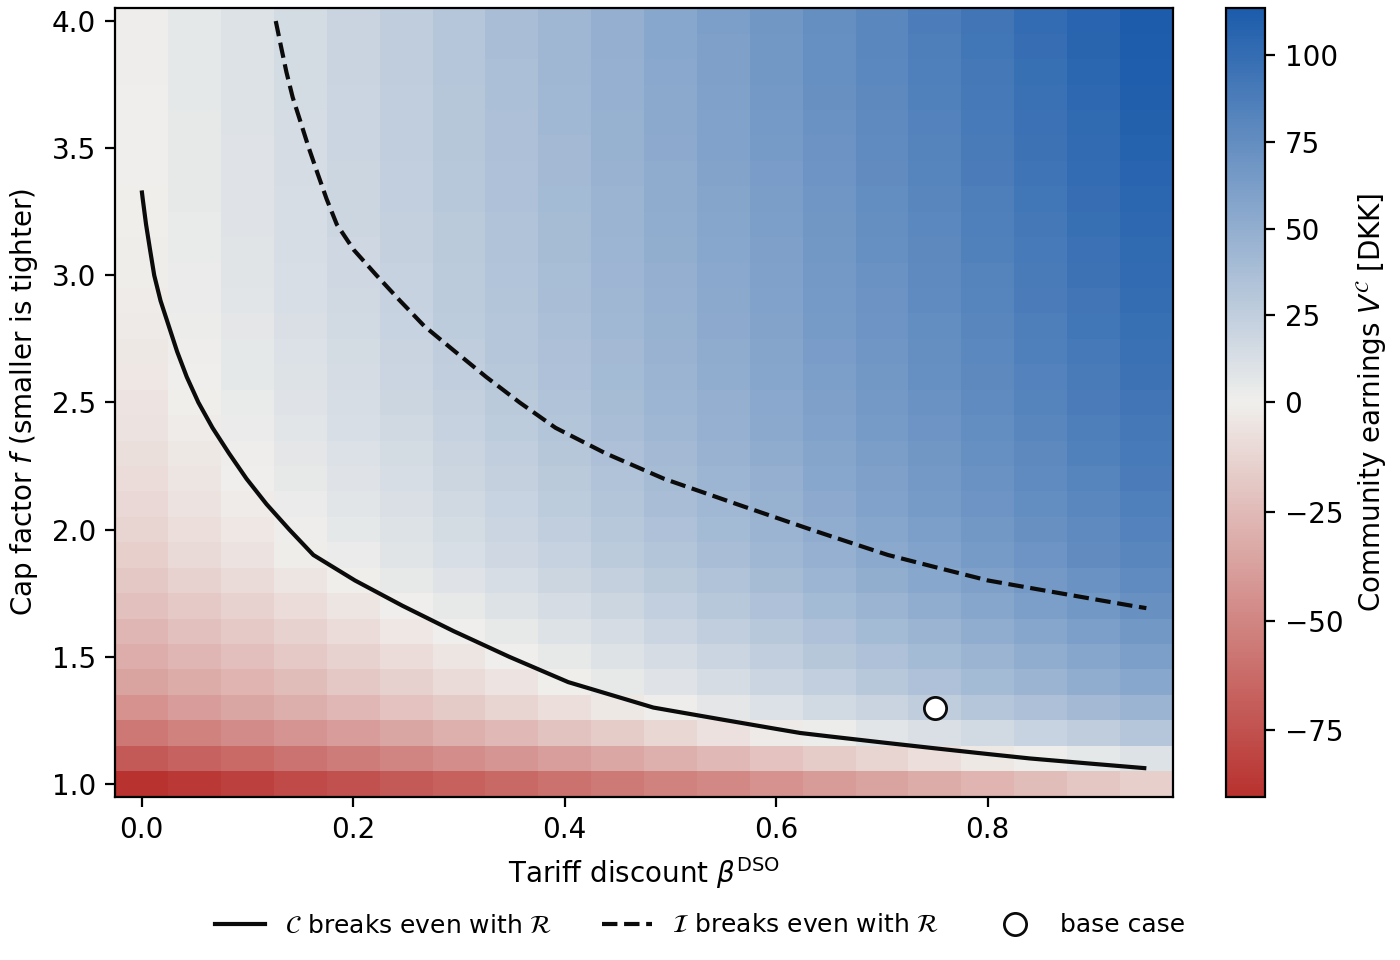
\includegraphics[width=0.8\linewidth]{figures/Q1/q1_sweep_earnings.png}
\caption{Community earnings $V^{\mathcal{C}}$ compared with $\mathcal{R}$. Blue means the community contract pays off}
\label{fig:sweep_earnings}
\end{figure}

Individual contracts only pay off above the dashed line in the dark blue region where the community contract already earns a lot.
They never pay off for $f\leq 1.6$ and still need a discount of 0.15 at $f=4.0$ where the cap no longer binds the community. Their slices thus keep binding some members.

Across all 620 combinations the flexibility of both contracts changes by less than 0.01~kWh with the discount. Figure~\ref{fig:sweep_flex} therefore shows flexibility against the cap factor alone. Due to the high penalty the community contract leaves less than 0.01~kWh above the cap in every combination. Its flexibility thus equals the congestion under $\mathcal{R}$. Individual contracts provide slightly less flexibility since each member is restricted separately rather than at the community level.
At the base cap they remove 62.1~kWh compared to 66.4~kWh for $\mathcal{C}$.
The two contracts provide equal flexibility for $f \geq 2.5$.
The DSO therefore gets nearly the same flexibility from both contracts.


\begin{figure}[htbp]
\centering
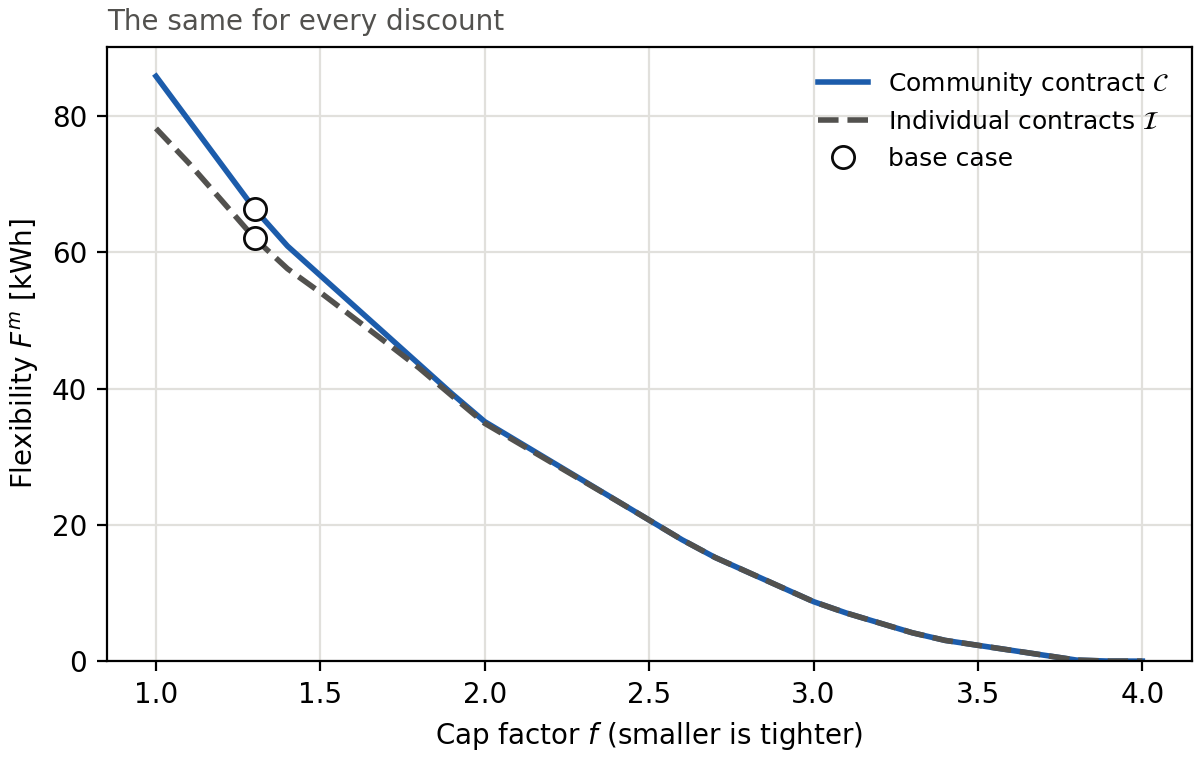
\includegraphics[width=0.7\linewidth]{figures/Q1/q1_sweep_flexibility.png}
\caption{Flexibility $F^m$ for the DSO. Both contracts give the same flexibility for every discount. Individual contracts remove slightly less when the cap is tight.}
\label{fig:sweep_flex}
\end{figure}

Together the two figures show the trade-off of the DSO.
The cap decides how much flexibility the DSO gets and the discount decides whether the community accepts.
From $f=2.0$ to $f=1.3$ the flexibility grows by 31.2~kWh for 0.35 more discount.
From $f=1.3$ to $f=1.1$ the same extra discount buys only 13.0~kWh.
Each extra kWh of flexibility thus becomes more expensive for the DSO as the cap tightens.

The figures thus confirm the hypotheses on the discount the community contract needs and on the flexibility.
The hypothesis on individual contracts holds only for the cap since a small discount is enough once the cap is loose.

\subsection{Settlement in $\mathcal{C}$}\label{sec:settlement}

The settlement is analysed on the base case of Section~\ref{basecase}, where the community contract $\mathcal{C}$ pays off for the community as a whole. This section shows whether every member also gains and whether the manager's budget is balanced. Under the settlement~\eqref{eq:payment}, all members pay the same internal price $\lambda_t$ in a given hour. This price is the dual of the balance~\eqref{eq:C_bal} and equals the cost to the community of one more kWh in hour $t$. It is unique in 23 of 24 hours. In the remaining hour no member consumes or produces energy, so its price affects no payment. Re-solving $\mathcal{C}$ with slightly more and slightly less consumption of each member gives the highest and lowest payment it could face. The two are equal for every member, so the results do not depend on which dual solution the solver returns.


In the hours where the cap binds and the community would like to import more, the internal price lies above the import price.
Since moving load to another hour is cheaper than the penalty, the community keeps its import at the cap.
One more kWh in such an hour therefore only fits if another member gives up its preferred schedule and moves one kWh out.
The internal price includes the discomfort of that member, making it the price at which the member is just willing to move.
In hour 11 even the stiff L4 loads must move, and the internal price reaches 5.41~DKK/kWh while the import itself costs only 1.225~DKK/kWh.

The manager collects 342.77~DKK at the internal prices but pays the DSO only 179.00~DKK at the discounted import price.
The difference of $B=163.77$~DKK stays with the manager, so the budget is not balanced.
Together the members thus lose 137.69~DKK, although the community as a whole gains 26.08~DKK.

\begin{figure}[H]
\centering
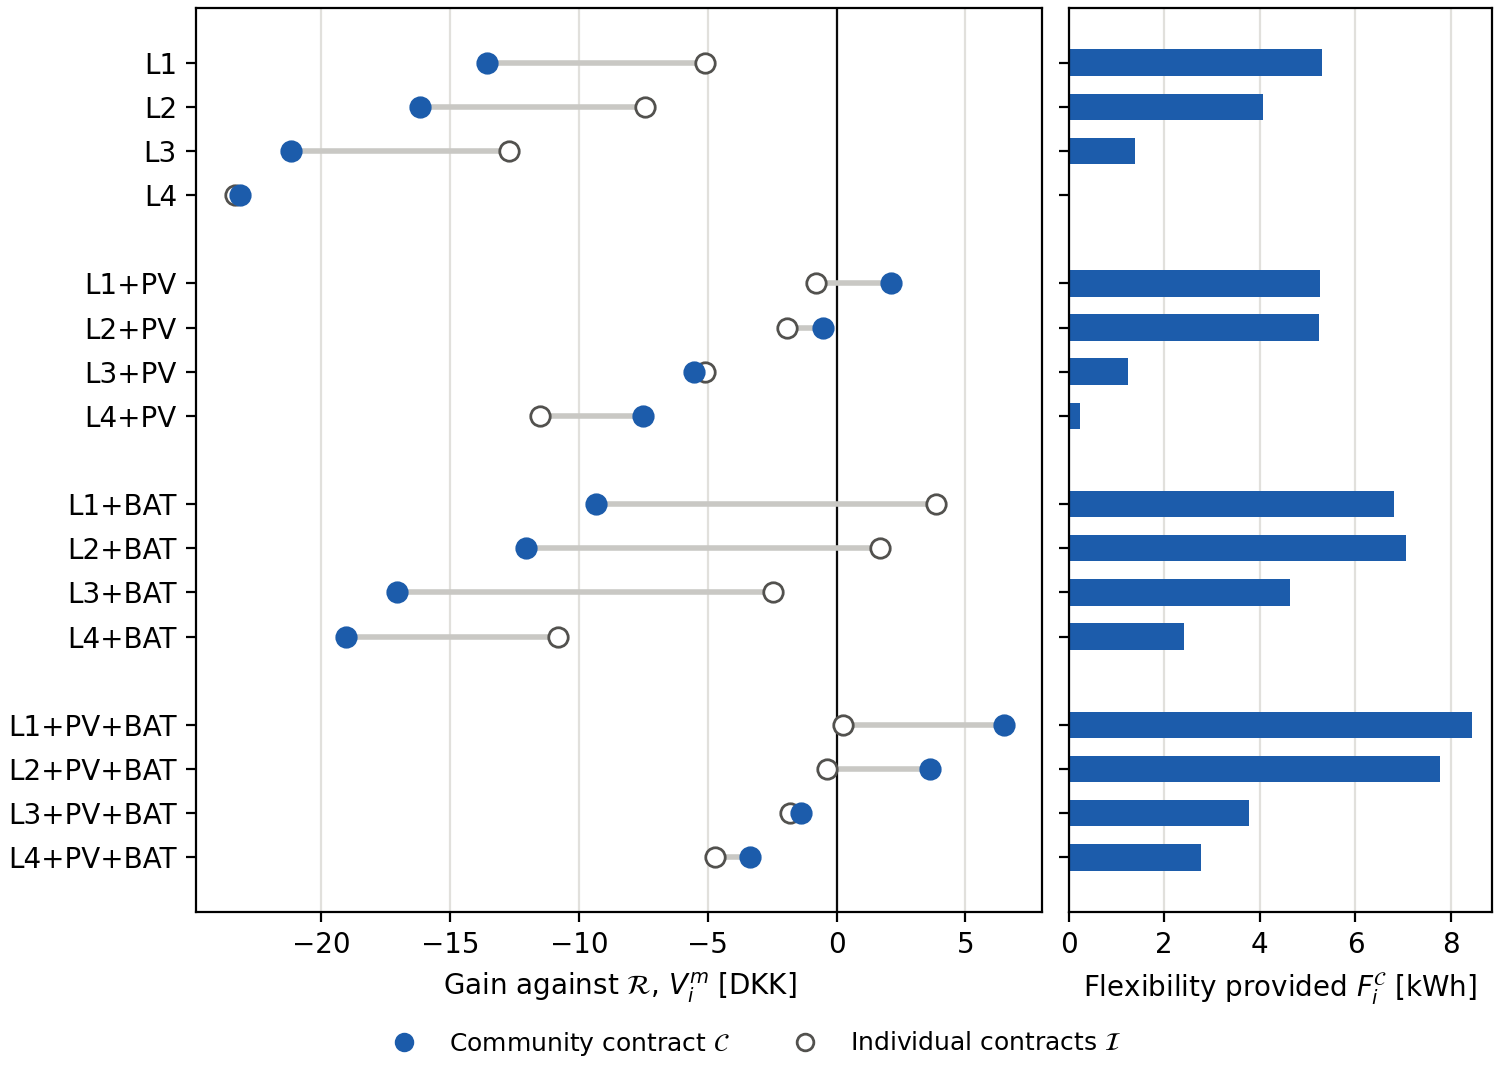
\includegraphics[width=0.85\linewidth]{figures/Q1/q1_settlement.png}
\caption{Gain of each member against $\mathcal{R}$ under the community contract (filled) and individual contracts (hollow), with the flexibility it provides in $\mathcal{C}$ (right).}
\label{fig:settlement}
\end{figure}

Figure~\ref{fig:settlement} shows the gain of every member compared with $\mathcal{R}$.
Only 3 of 16 members are not worse off than $\mathcal{R}$, and all of them own PV and have a flexible load(L1 or L2).
They sell PV energy to other members at the high internal price.
Members who cannot move their load still pay this price, as it is the same for everyone.
The stiff L4 member without assets therefore loses the most with 23.16~DKK.
Compared with $\mathcal{I}$, 8 of 16 members are not worse off under $\mathcal{C}$. All battery owners without PV would however prefer $\mathcal{I}$. These battery owners provide 5.23~kWh of flexibility on average but still lose 14.38~DKK. This is probably because the battery is worth less to its owner in $\mathcal{C}$. In $\mathcal{I}$ it saves the penalty on the owner's own small cap.
In $\mathcal{C}$ the cap is shared, so the battery competes with the flexibility of all other members and only earns the spread of the internal price.

PV owners without battery provide only 2.99~kWh and lose just 2.86~DKK.
Under the dual settlement, owning PV thus matters more than providing flexibility.

\subsection{Summary and Recommendations}
This section summarizes the main findings and gives recommendations to the members, manager and DSO.

Figure~\ref{fig:settlement} shows that an individual contract is the best option for only two members, the L1 and L2 members with only a battery. Since all members take the same decision, individual contracts are still not relevant as they cost the community 82.4~DKK and never pay off for $f\leq 1.6$ in Section~\ref{sec:sensitivity}. The community contract is the best option for three members, the L1 member with PV and the L1 and L2 members with PV and battery. It earns the community as a whole 26.08~DKK, but the other 13 members lose under it as the manager keeps a surplus of 163.77~DKK. A community contract therefore needs a joint decision that binds every member, since those who prefer $\mathcal{I}$ or $\mathcal{R}$ would otherwise refuse it. For 11 of 16 members $\mathcal{R}$ is the best option, so a majority vote would keep the members in $\mathcal{R}$ under the current settlement. The community contract would only become relevant if the manager paid the surplus back to the members in some fitting way. As the community gains as a whole, such a repayment could compensate every member who loses. 

The manager prefers the community contract, as it keeps the surplus of 163.77~DKK. Compensating the 13 members who lose would cost 149.92~DKK, so the manager would still keep 13.85~DKK in that case. Sharing part of the surplus can therefore suit both the manager and the members.

The goal of the DSO is to remove enough congestion at the lowest possible discount. Section~\ref{sec:sensitivity} shows that a tighter cap gives more flexibility but requires a larger discount, from 0.50 at $f=1.3$ to 0.85 at $f=1.1$. At $f=1.0$ no discount up to 0.95 is enough. The DSO should therefore choose the loosest cap that still relieves its feeder the desired amount, with a discount just large enough for the community to be formed. This only holds if the manager shares the surplus, as the members would otherwise not sign.
.



